\section{Introduction}
\label{S:Intro}


The automated exploration of unknown environments has become one of the foremost challenges in mobile robotics. For a robot to explore an environment, it must map the environment and concurrently localize itself within said environment.  The framework used to perform this task is known as simultaneous localization and mapping (SLAM) and has been well covered in the literature using a variety of techniques \cite{durrant2006simultaneous,bailey2006simultaneous}.

While SLAM is well known and has a rich history of successes using a single robot, it can often be a slow process due to both constraints on the robot, such as speed and data processing, and lack of redundancy, i.e. robot failure \cite{thrun2001probabilistic,burgard2005coordinated}.  To address the speed of mapping and to add redundancy, coordinated or multi-robot SLAM (MRSLAM) was created.

MRSLAM is as it sounds, SLAM using multiple exploring/mapping robots. This approach allows for the partition of the physical search space using independent robots, typically decreasing the time it takes to map an area, and increasing the likelihood of full map coverage in the event of robot failure. This temporal exploration parallelism does, however, come at the cost of added complexity. The added complexity of MRSLAM comes in two major components: coordination of exploration using multiple search agents and merging the maps of these agents \cite{fox2006distributed}.  Coordinated exploration consists of planning the groups' search path, most often formulated to cover the most search space in minimum time or to optimize some other mapping cost criteria. The other major component, map merging, is the combination of individual robot's observations and maps into one cohesive global map estimate.

In this paper we use the map merging algorithm presented in Howard's 2006 paper: ``Multi-Robot Simultaneous Localization and Mapping using Particle Filters'' \cite{howard2006multi}. This paper is of particular interest as it presents a resource efficient, online solution to the MRSLAM map merging problem given unknown initial robot poses.  

The algorithm is an encounter-based algorithm.  Given that we start with one mapping robot (call this Robot 1), when it encounters a non-mapping robot (Robot 2), the relative pose between the two robots is computed and Robot 2's odometry and measurement data is transmitted in reverse order to Robot 1 and integrated to create a single map posterior.  

Fig. \ref{fig:HowardFig3} depicts the process with Robot 1's triple $(\textbf{x}^1_t,u^1_{t-1},z^1_t)$, and robot 2's triple $(\textbf{x}^2_t,u^2_{t-1},z^2_t)$, building a single global map posterior $m$.
When $t=2$, Robot 1 observes Robot 2 and determines the relative pose $\Delta$, then the past odometry and scan data is integrated in reverse order.

\begin{figure}[h]
\centering
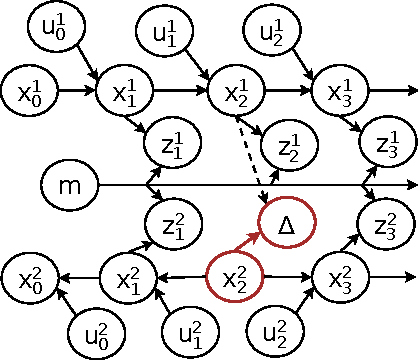
\includegraphics[width=\columnwidth]{{{../FinalFigures/HowardFig3}}}
\caption{Depiction of data integration. Taken from \cite{howard2006multi}.}
\label{fig:HowardFig3}
\end{figure}

While Howard's method is attractive for its speed, it combines the forward and reverse particle weights, which can result in undesired particle error.  In this paper we propose a modification of the algorithm by using independent particle filters for each robot, and demonstrate that the modified algorithm provides a qualitatively better map, and a more accurate pose estimate.

The paper is structured as follows: In \S\ref{S:Back} some background about MRSLAM is provided, the contribution of \cite{howard2006multi} is discussed and a modified scheme is presented.  In \S\ref{S:Alg} the modification of Howard's algorithm \cite{howard2006multi} is discussed.  In \S\ref{S:Exp} the generation of arbitrary data sets, the average time it takes to map 95\% of the environment, and a comparison of Howard's algorithm and the modified algorithm are presented.  \S\ref{S:Conc} rounds out the paper with conclusions and future work.

